\chapter{Main controller}
\section{Inleiding}
De main controller bevat de interface van de wekker. Deze zorgt er voor dat een wekker ingesteld kan worden, aangepast kan worden en uitgezet kan worden. 
Belangrijk aan elke interface is dat deze gebruiksvriendelijk is. 
Dit kan onder andere bereikt worden door een optimum voor het aantal knoppen te bepalen. 
Te veel knoppen, en de gebruiker weet niet welke knop wat doet, te weinig knoppen, en de gebruiker moet navigeren door een nodeloos ingewikkeld menu. \\
Daarnaast is er nog een beperkende factor: het aantal pinnen op de chip. \\
Dit alles bijeengenomen leverde een zo gebruiksvriendelijk mogelijke interface als er gebruik word gemaakt van 4 knoppen. Daarnaast is er nog een knop die slechts gebruikt wordt om een afgaand alarm uit te zetten. \\
De controller stuurt een hoop dingen aan, en van te voren was al geanticipeerd dat dit hierdoor een van de grootste onderdelen op de chip zou kunnen worden.

\section{Specificaties}
De controller moet aan een aantal eisen voldoen zodat andere componten overweg kunnen met de uitgangsignalen van de controller. De tijd moet gecodeerd worden volgens het DCB codering. Om door te geven of het alarm of onderelen aan of uit zijn wordt gebruik gemaakt van positieve logica. Dit houd in als er een $1$ als uitgangsignaal is dan staat het onderdeel aan. Het reset gebeurt bij een hoog signaal en synchroon met de klok.

\subsection{Ingangen}
\begin{itemize}[nolistsep]
\item Klok, dit is een standaard input;
\item Reset, ook dit is een standaard input;
\item Knoppen, dit zijn de 4 knoppen die (nadat ze gebufferd zijn) onderdeel zijn van de interface.
\begin{itemize}[nolistsep]
\item knoppen[0] = menu
\item knoppen[1] = set 
\item knoppen[2] = up
\item knoppen[3] = down\\
\end{itemize}
\end{itemize}



\subsection{Uitgangen}
\begin{itemize}[nolistsep]
\item Wekker, dit is een vector van 16 lang. In dit signaal zijn alle instellelingen te vineden van hoelaat de wekker afgaat tot of het alarm aan of uit is.
\item Menu, een vector van 3 lang hierin is gecodeerd welke state de gebruiker is zodat de lcd de output eraan kan aanpassen.\\
\end{itemize}
In \cref{tab:uitgangen_controller} staat wat voor informatie te vinden is in de uitgangen van de controller.
\begin{table}[ht!]
\caption{Uitgangen van de controller}
\label{tab:uitgangen_controller}
\begin{tabular}{|p{.25\textwidth}| p{.75\textwidth}|}
\hline
Uitgang & Informatie over wat in de uitgang te vinden is \\ \hline
wekker & De huidige info over de wekker instellingen uit geheugen \newline
wekker[6 down to 0] daarin staan de minuten \newline
wekker[12 down to 7] daarin staan de uren \newline
wekker[13] geluid bit \newline
wekker[14] led bit \newline
wekker[15] wekker bit (Of de wekker uberhaupt aan is of niet) \\ \hline
menu & Deze geeft door aan de in welke state we zitten aan de lcd module \newline
000 : Het normale scherm weergeven met alarm en wekkertijd weergave states : (Rust, wekker toggle \newline
001 : Uren aanpassen states : (uren set, uren min/plus) \newline
010 : Minuten aanpassen states : (minuten  set, minuten min/plus) \newline
011 : Led aanpassen states : (Led, Led toggle)\newline
100 : Geluid aanpassen states : (Geluid, Geluid toggle)\newline
101 : De menu is geopend states : (Wekkertijd)\\ \hline
\end{tabular}
\end{table}
\newpage
\subsection{Gedrag}
Om te beginnen moet de tijd waarop de wekker af gaat ingesteld kunnen worden. Dit wordt gedaan door eerst de huidige wekkertijd weer te geven, vervolgens het uur waarop gewekt moet worden te wijzigen en daarna de minuten. Hierna wordt de huidige tijd weer weergegeven. \\
Daarnaast is een vereiste dat de alarm in het geheel of gedeeltelijk uitgezet kan worden. Afhankelijk van een instelling moet het niks gebeuren of een combinatie van het afgaan van de led en geluid.\\
Dit alles moet gebruiksvriendelijk mogelijk zijn.

\section{Functionaliteit}

Om de controller goed hi\"{e}rarchisch te kunnen ontwerpen is deze opgedeeld in 3 componenten.
Een buffer voor de vier knoppen, geheugenelement en het menu zelf. In \cref{fig:blk_controller} is te vinden hoe de blok diagram van de controller eruit ziet.

\begin{figure}
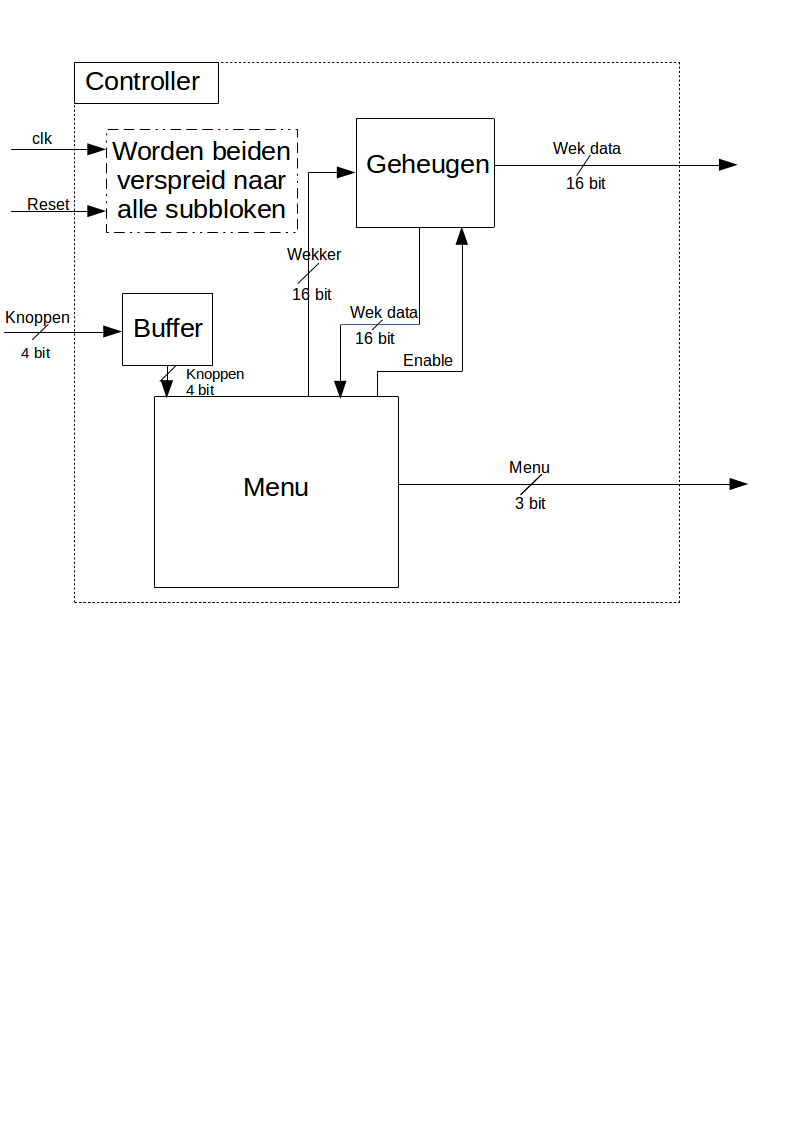
\includegraphics[width=\textwidth,height=\textheight,keepaspectratio]{Figuren/Controller/blok_controller.png}
\caption{Blok diagramma van de controller}
\label{fig:blk_controller}
\end{figure}

Voor het menu is een grote FSM die in \cref{fig:FSM_controller} staat de gemaakte fsm en in \cref{tab:states_controller} staan de uitgangen per state gespecificeerd. 

\begin{figure}[ht!]
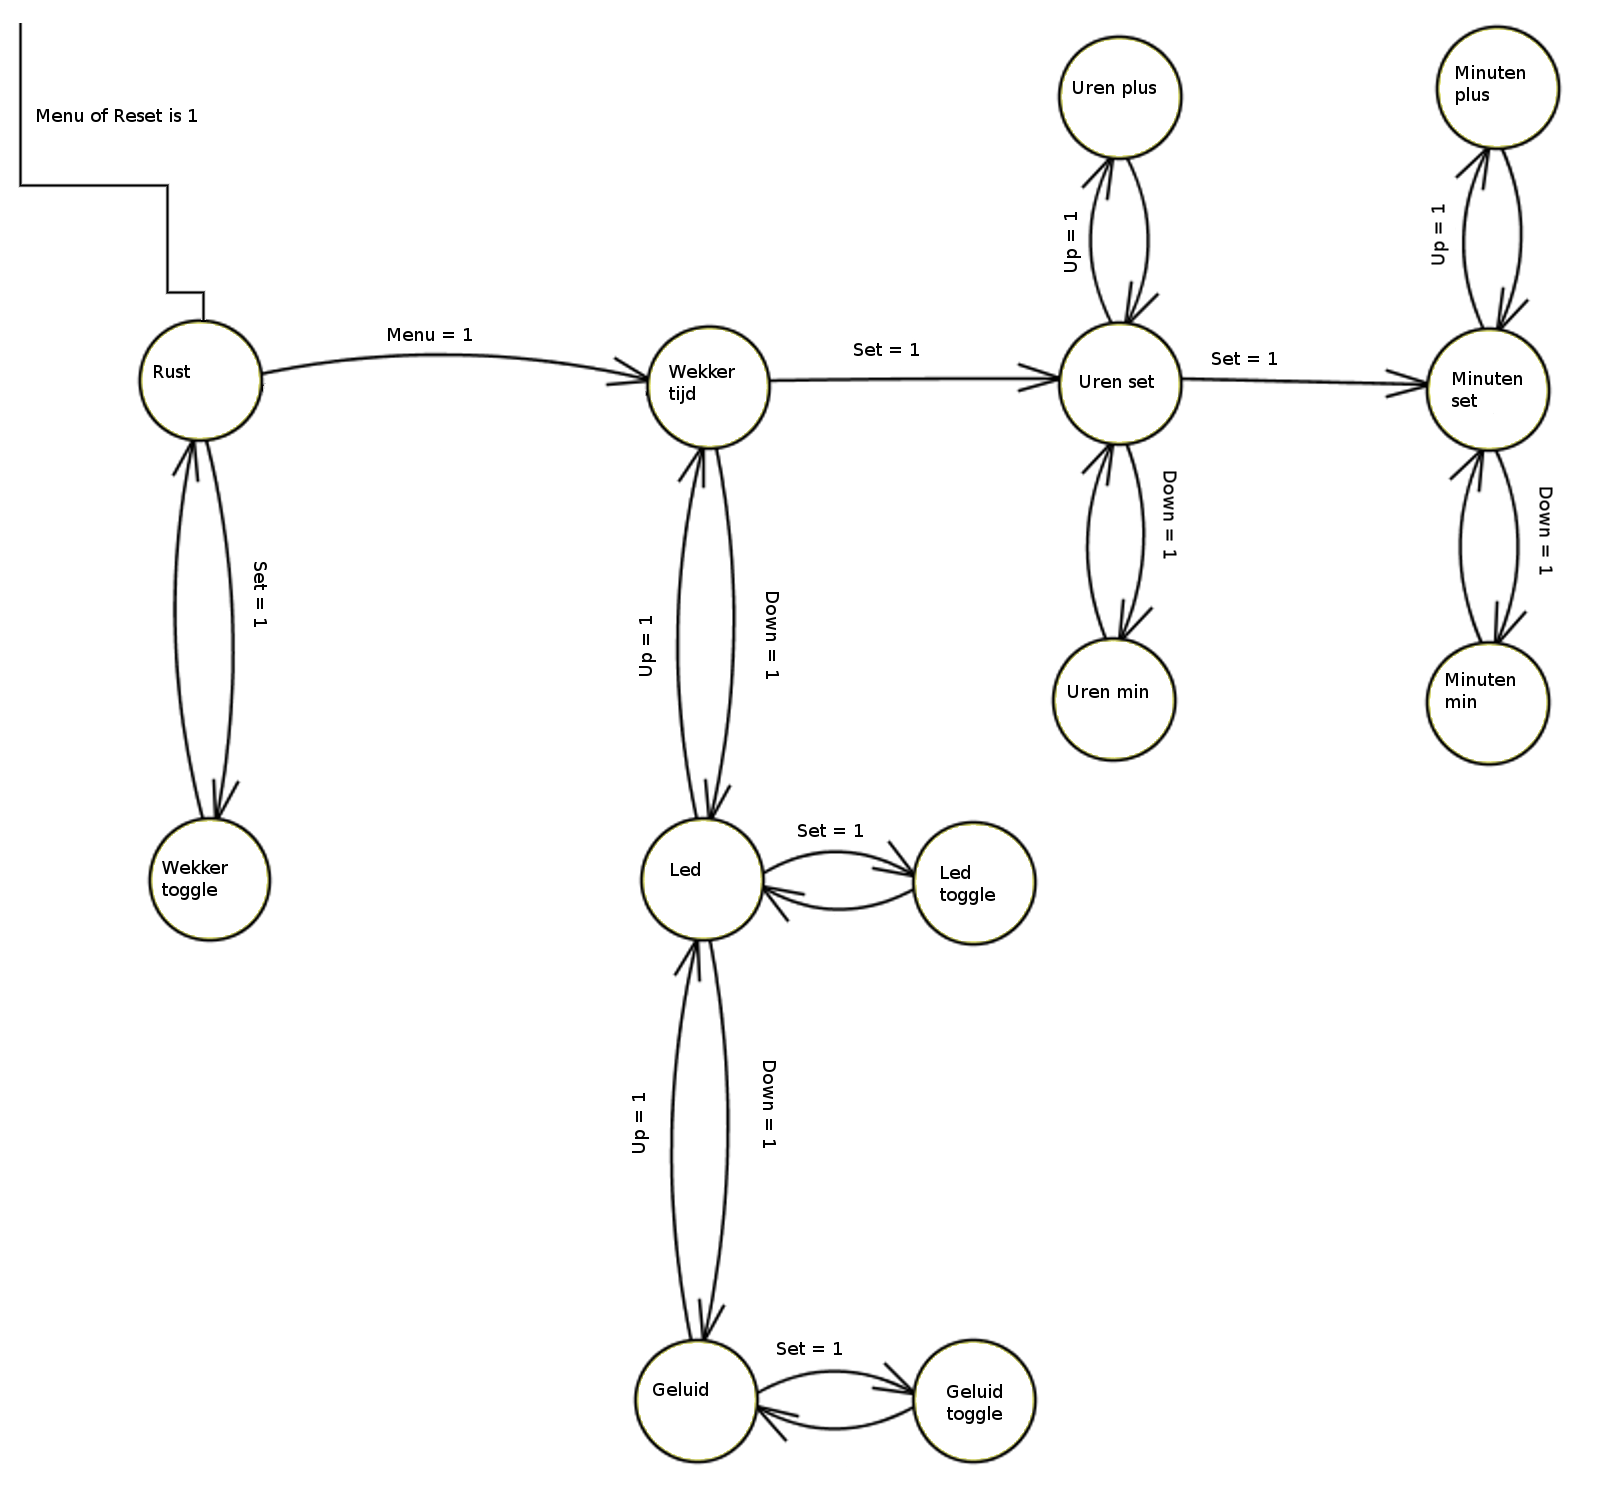
\includegraphics[width=\textwidth,height=\textheight,keepaspectratio]{Figuren/Controller/FSM_controller.png}
\caption{FSM diagramma van de menu}
\label{fig:FSM_controller}
\end{figure}

\begin{longtable}{|p{.25\textwidth}| p{.75\textwidth}|}
\hline
Rust &
enable = '0' \newline
wekker=wekdata \newline
menu= "000" \\ \hline
Wekker toggle &
enable = '1' \newline
wekker[12 down to 0]=wekdata[12 down to 0] \newline
wekker[13]= niet wekdata[13] \newline
menu = "000" \\ \hline
Wekkertijd &
enable ='0' \newline
wekker=wekdata \newline
menu = "000" \\ \hline
Led &
enable ='0' \newline
wekker=wekdata \newline
menu = "011" \\ \hline
Led toggle &
enable ='1' \newline
wekker[11 down to 0]=wekdata[11 down to 0]\newline
wekker[12] = niet wekdata[12] \newline
wekker[13] = wekdata[13] \newline
menu = "011" \\ \hline
Geluid & 
enable ='0' \newline
wekker=wekdata \newline
menu = "100" \\ \hline
Geluid toggle &
enable ='1' \newline
wekker[10 down to 0]=wekdata[10 down to 0] \newline
wekker[11] = niet wekdata[11] \newline
wekker[13 downto 12] = wekdata[13 downto 12] \newline
menu = "100" \\ \hline
Uren set &
enable ='0' \newline
wekker=wekdata \newline
menu = "001" \\ \hline
Uren plus &
enable ='1' \newline
wekker=wekdata+1 \newline
menu = "001" \\ \hline
Uren min &
enable ='1' \newline
wekker=wekdata-1 \newline
menu = "001" \\ \hline
Minuten set&
enable ='0' \newline
wekker=wekdata \newline
menu = "010" \\ \hline
Minuten plus &
enable ='1' \newline
wekker=wekdata+1 \newline
menu = "010" \\ \hline
Minuten min &
enable ='1' \newline
wekker=wekdata-1 \newline
menu = "010" \\ \hline
\caption{Uitgangen binnen de state van de controller} 
\label{tab:states_controller}
\end{longtable}

\section{VHDL code}
De code voor de controller van de wekker is te vinden in \cref{Ap:code_controller}. Voor de overzicht en het modular opbouwen is de code in vier blokken geschreven.
\begin{itemize}[nolistsep]
\item De top entity met de port map. Deze is te vinden in \cref{code:controller_ent,code:controller_beh}.
\item Het menu, hierin zit de echte logica verwerkt. Deze is te vinden in \cref{code:menu_ent,code:menu_beh}.
\item Het gebruikte geheugen element voor de opslag van 16 bits, te vinden in \cref{code:geheugen_ent,code:geheugen_beh}.
\item De gebruikte buffer is te vinden in \cref{code:buffer_ent,code:buffer_beh}. De buffer regelt het ingangssignaal, en zorgt ervoor dat er maar 1 klokperiode lang een hoog signaal gelezen word.
\end{itemize}
Voor het testen van de code zijn er testbenches gemaakt welke te vind zijn in \cref{code:tb_controller,code:tb_menu,code:tb_geheugen,code:tb_buffer}.

\section{Testen}
Om zeker te zijn dat alles goed werkt worden er vier verschillende testen uitgevoerd. De belangrijkste zijn de behavoural en switch level simulatie. Om zeker te zijn dat alles goed werkt wordt er ook nog een test gedaan door de code te synthetiseren en te extracten uit de schakeling.
Bij een test op behavioural niveau wordt er gekeken of de code werkt zoals verwacht. Na een geslaagd resultaat kan de code worden gesynthetiseerd, en deze gesynthetiseerde code worden gesimuleerd. Als er geen fouten optreden kan het ontwerp gemaakt worden, daarna ge\"{e}xtraheerd en nogmaals getest worden. De testen worden uitgevoerd met behulp van \emph{Modelsim}. De laatste stap bevat de switch level simulatie deze is als bijlage ingeleverd bij het document.


\section{Simulatie}
De resultaten van de simulatie staan in \cref{Ap:sim_controller}. De testbench is te lang om in een keer weer te geven daarom is deze op geknipt in vier stukken. De testbench die gemaakt is voor de simulatie staat in \cref{code:tb_controller}
\section{Resultaten}
Van \cref{fig:sim_beh_0-2_5} tot en met \cref{fig:sim_ext_7_5-} is te zien dat iedere simulatie tot hetzelde resultaat leid en daarmee succesvol is.
De minimale klokperiode kan afgelezen worden aan de hand van \cref{fig:timing_controller}. Hieruit is op te makken dat deze 60ns is.
\subsection{Conclusie en discussie}
De controller werkt op alle gesimuleerde niveau's naar verwachting. Voor een correcte werking heeft de controller een klok periode die volgens de simulaties ten minste 60ns moet bedragen om gliches te voorkomen
De controller maakt gebruik van 8606 transitoren waarvan er voor de daadwerkelijke logica slechts 2965 worden gebruikt. Vlak nadat het inputbuffer gemaakt was kwam men er achter dat in plaats van een buffer ook de \emph{rising\textunderscore edge} functie gebruikt had kunnen worden. Hier is niet voor gekozen omdat het dan niet altijd even duidelijk is wat er gebeurd als er twee knoppen tegelijk ingedrukt worden.

